\begin{problem}{GPUs \& CUDA Framework \hfill[15 pts]}{prob:gpu}

    As mentioned in Lectures I and III, GPUs have transformed neural network training by enabling massive task parallelization. This problem aims to introduce some fundamental concepts of GPU programming and its application to deep learning.

    \vspace{10px}
    \textbf{Background \& Definitions}

    A byproduct of their original purpose, GPUs are inherently optimized for massively parallel tasks, making them ideal for deep learning computations. Unlike CPUs, which typically have a single-to-double digit count of highly optimized cores, GPUs contain thousands of smaller cores optimized for high-throughput parallel processing.
    To gain a preliminary understanding of their importance and how they can be used to accelerate neural networks, we will briefly delve into Nvidia's  CUDA platform, the most widely used platform for GPU programming. 
    
    \begin{enumerate}
        \item \textbf{CUDA}: \textit{(Compute Unified Device Architecture)} is a programming model developed for Nvidia's GPUs which allows users to write kernels and manage data transfer between the ``host" (CPU) and ``device" (GPU). The CUDA environment is C/C\texttt{++}-like*, but we'll be using the Python library \href{https://pypi.org/project/pycuda/#description}{\tt pyCUDA} to interface with the APIs.
        \item \textbf{Kernel}: A computation-performing function that runs on the GPU. Kernels are launched on the device and run on multiple threads simultaneously. 
        \item \textbf{Thread}: The fundamental unit of work within a kernel, which usually perform the same operation across different data. 
        \item \textbf{Block}: A group of threads that execute together on the GPU, logically unified by a self-contained shared memory pool. Blocks are isolated from one-another. 
        \item \textbf{Grid}: A virtualized collection of blocks that execute a kernel. Grids can be structured in 1 to 3 dimensions to represent parallel problems.
    \end{enumerate}
        \begin{figure}[H]
        \centering
        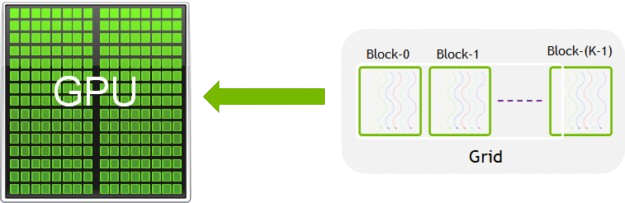
\includegraphics[width=\linewidth]{media/viz_blocks_grid.png}
        \caption{Visual representation of the CUDA hierarchy. \cite{Gupta_2023}}
        \label{cuda diagram}
    \end{figure}
    *Don't worry if you've never been exposed to C\texttt{++}, the syntax is essentially the same as C or Java, and you won't be doing anything too complicated. If your background is solely Python \href{https://web.stanford.edu/class/archive/cs/cs106b/cs106b.1252/resources/python_to_cpp.html}{here's a short guide with all the syntax you'll need}. Additionally, a small section on interfacing with pointers is included in the Colab.

    \newpage
    \textbf{Indexing Inside a Kernel}

    This hierarchy of \textbf{grid}, \textbf{block}, and \textbf{thread} forms the foundation of GPU programming, enabling organized parallel computations. But how can we use this for parallel processing?

    \vspace{10px}
    Every thread has a unique identifier, which can be determined by its position within its block, and the position of its block within the grid. By using these identifiers, threads can independently process data in a manner that corresponds to their specific task in parallel. The CUDA runtime provides these through the variables below, which are made available within any kernel that you write.

    \begin{itemize}
        \item \texttt{threadIdx.x}, \texttt{threadIdx.y}, \texttt{threadIdx.z}: A thread's index within its block in the x, y, and z dimension.
        \item \texttt{blockIdx.x}, \texttt{blockIdx.y}, \texttt{blockIdx.z}: A block's index within the grid along respective dimension.
        \item \texttt{blockDim.x}, \texttt{blockDim.y}, \texttt{blockDim.z}: \# total threads in each block along respective dimension.
        \item \texttt{gridDim.x}, \texttt{gridDim.y}, \texttt{gridDim.z}: \# blocks in grid across respective dimension. 
    \end{itemize}

    When launching a kernel with pyCUDA, we specify both the block size, \texttt{block}, and the grid size, \texttt{grid} we want to use to ensure we sufficiently cover the size of the input data. We will stick to a block size of $16 \times 16 \times 1$, and define our grid size based on the block size as and the size of the data.

    \vspace{10px}
    Using these variables, we can map locations in memory to physical hardware cores. As this problem will deal with 2D structures only, you'll only need to use the following lines of code.

    \begin{verbatim}
    int idx = threadIdx.x+blockDim.x*blockIdx.x;
    int idy = threadIdx.y+blockDim.y*blockIdx.y;\end{verbatim}
    There are of course, tons of additional systems-level and hardware-level details, but for this problem the only other detail you need to know is that GPUs have their global memory (VRAM), which is larger yet slower to access than the shared memory available to a given block.

    \vspace{10px}
    \textbf{General CUDA Workflow}

    Now, let's cover the typical framework to follow once you've established that a problem can be solved in parallel with a guided example. Create a copy of the Google Colab environment for this project \href{https://colab.research.google.com/drive/1Y38N7kXJuTd-TPAA5fzQLVsc25rI9Qkc?usp=sharing}{linked here} and follow along until you reach the next section.

    \newpage
    \textbf{Matrix Multiplication Kernel}
    
    Now, it's your turn to dive deeper.
    \vspace{10px}
    
    Matrix operations are a necessity at every step of training a deep learning model, from data augmentation to neuron activations and backpropagation. By definition, linear operators are distributive, and thus most of the matrix operations used behind the scenes of deep learning are known as \textit{embarrasingly parallel} problems, since individual operations can be computed independently and brought together after.

    \vspace{10px}

    Your task is to implement a kernel to compute the matrix multiplication 
    \begin{gather*}
        C = AB \\
        dim(A) = n \times m \\
        dim(B) = m \times p
    \end{gather*}
    
    \vspace{10px}
    
    Hint, recall the dot product definition of matrix multiplication
    \[
        C_{ij} = \sum_{k=1}^{m} A_{ik} \cdot B_{kj}
    \]

    \vspace{10px}
    \textbf{Tasks}
    \begin{enumerate}
        \item Include a shareable link to your Colab. \hfill (required)
        \item Write down how long it takes for your \texttt{doublify} kernel to execute for $n=2^{12}$. \hfill (2 pts)
        \item Copy the benchmarks graph you made for your \texttt{matmul} kernel, and describe the runtime trends you see. \hfill (10 pts)
        \item Explain (don't implement) 2 nontrivial* ways your \texttt{matmul} kernel could be optimized for speed. This can be either software or hardware-dependent. \hfill (3 pts)

    \end{enumerate}

    If you liked this problem, consider reading through \href{http://courses.cms.caltech.edu/cs179/}{CS179}'s course materials.
    
    
\end{problem}


\begin{solution*}{}{}
\begin{enumerate}
    \item \href{https://colab.research.google.com/drive/10ih_KraR17stg4llNfxWk82pU-lto32N?usp=sharing}{colab link}
\item Kernel Speed: 0.000663 seconds
\item The runtime grows exponentially with matrix size for both methods, and the
    gpu runs twice as fast for large matrix sizes (8192 and 16384).
\begin{center}
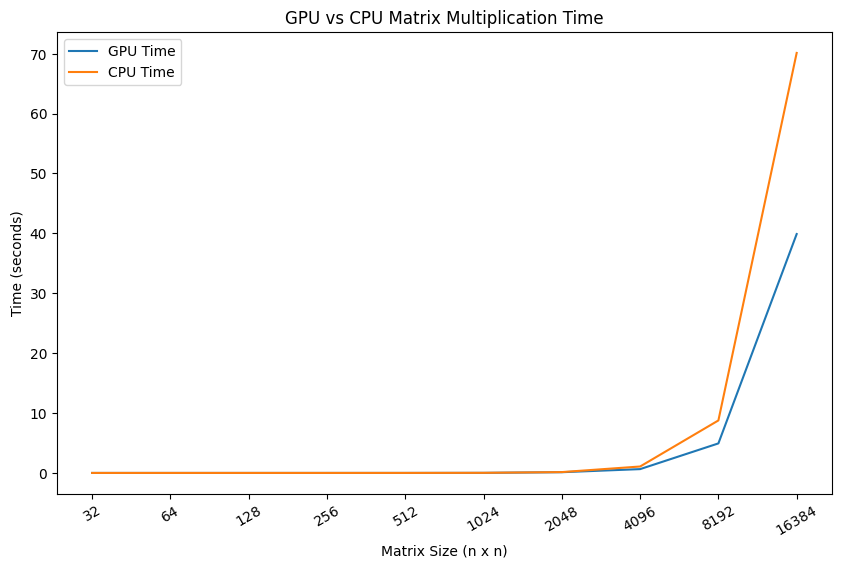
\includegraphics[width=0.8\textwidth]{media/5.png}
\end{center}
\item To make it faster, we can store $B$ as $B^{T}$ instead the GPU caches rows
    of values together as they are closer together in the 1D flattened array,
    and thus are likely to be cached together when accessed (I know this is true
    for CPUs at least from CS 24). We can also load the memory for the
    corresponding blocks into the shared memory so there's no transfer speed
    delay and use TPUs.
\end{enumerate}
\end{solution*}
